\section{Analysis}

The model outperforms the average cardiologist score on both the sequence and
the set F1 metrics. Figure~\ref{fig:arrhythmias:model_confusion} shows a
confusion matrix of the model predictions on the test set. Many arrhythmias are
confused with the sinus rhythm. We expect that part of this is due to the
sometimes ambiguous location of the exact onset and offset of the arrhythmia in
the ECG record. Figure~\ref{fig:arrhythmias:human_confusion} shows a confusion
matrix for the individual cardiologists on the test set. The high-level
structure of the two confusion matrices is similar, suggesting that the model
and cardiologists tend to make the same mistakes.

\begin{figure}
\begin{subfigure}{.5\textwidth}
  \centering
  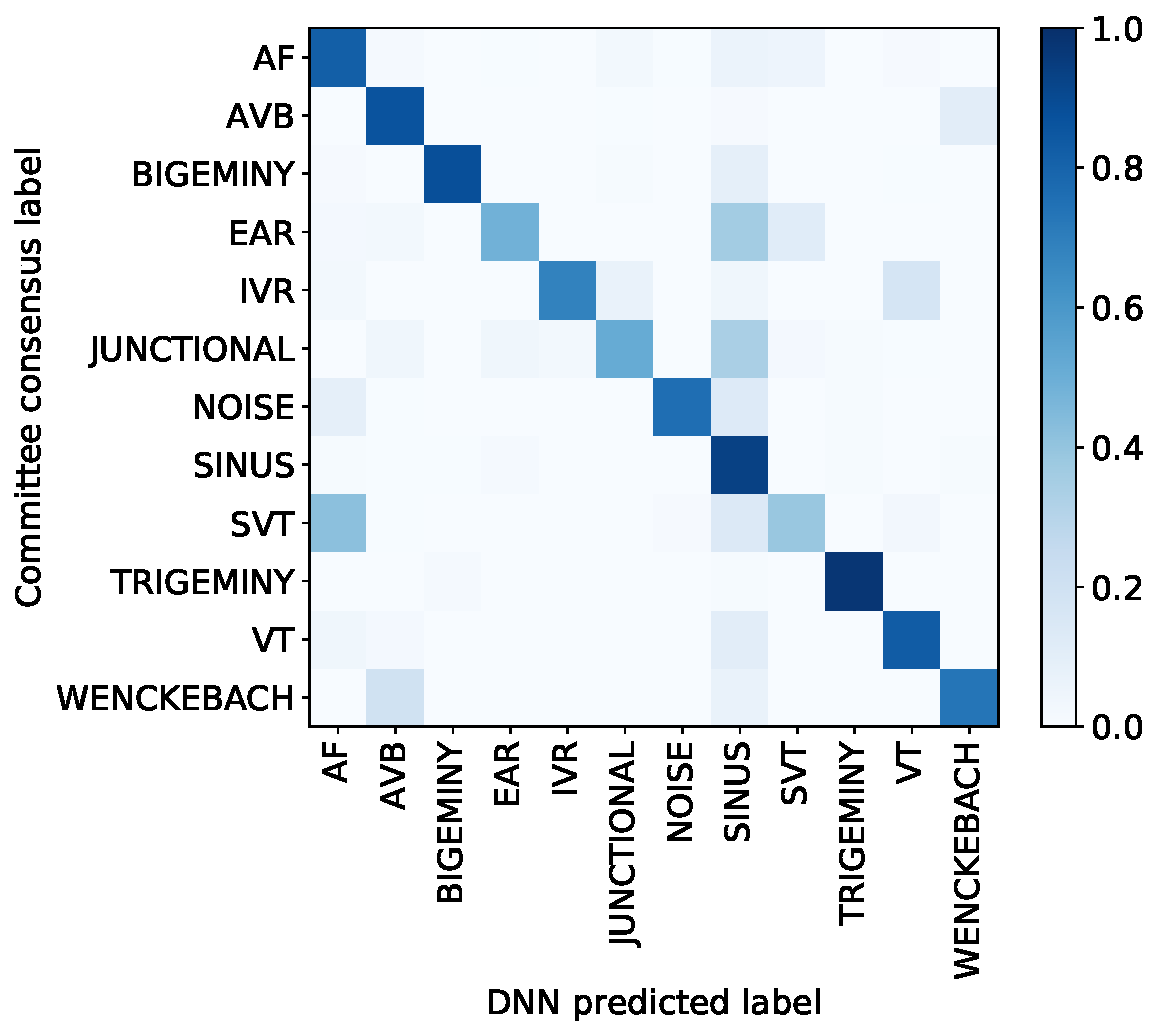
\includegraphics[width=0.9\linewidth]{arrhythmias/figures/model_confusions.pdf}
  \caption{Model}
  \label{fig:arrhythmias:model_confusion}
\end{subfigure}
\begin{subfigure}{.5\textwidth}
  \centering
  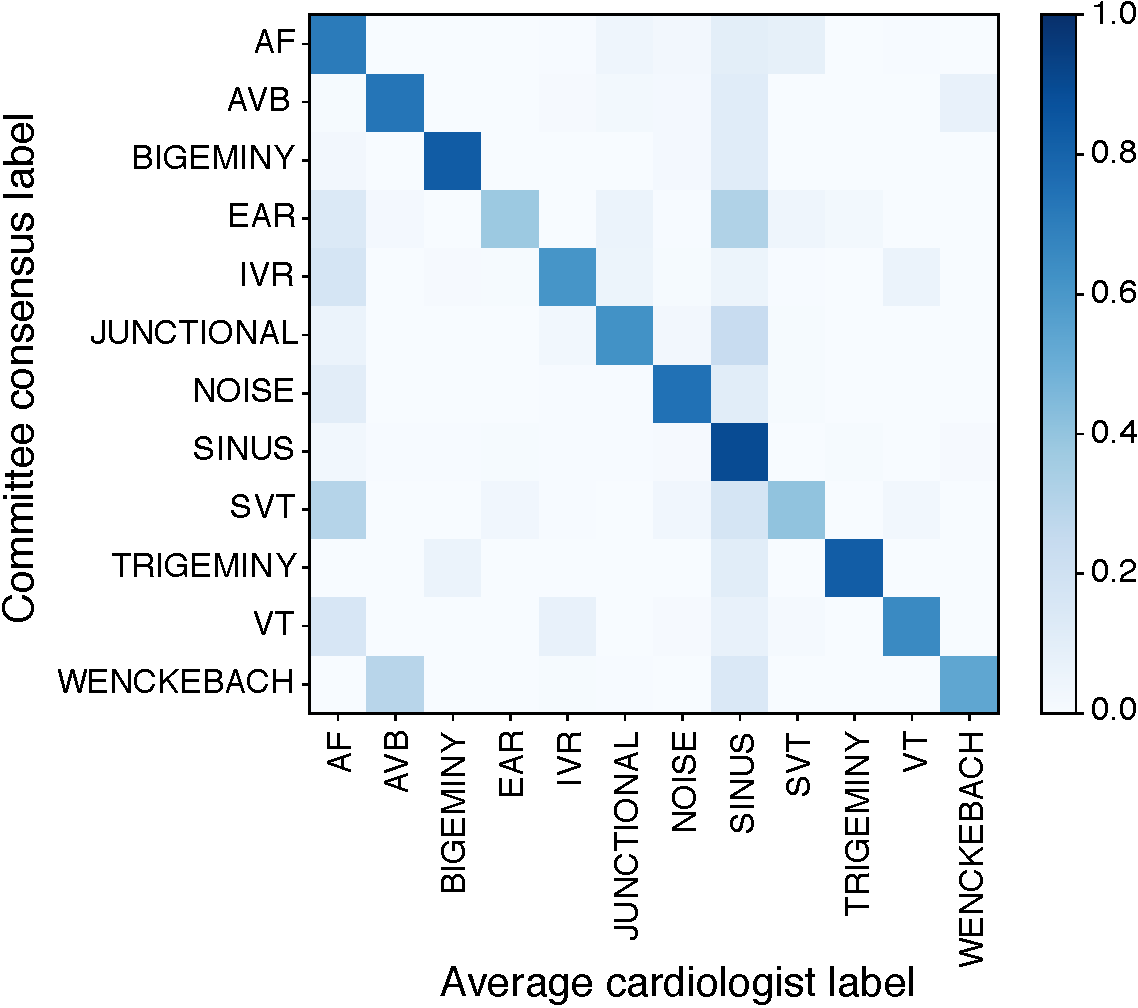
\includegraphics[width=0.9\linewidth]{arrhythmias/figures/human_confusions.pdf}
  \caption{Individual Cardiologists}
  \label{fig:arrhythmias:human_confusion}
\end{subfigure}
\caption{Confusion matrices for the model and individual cardiologist
         predictions with the committee consensus annotations as ground
         truth.}
\end{figure}

Often the mistakes made by the model are understandable. For example, confusing
Wenckebach and AVB makes sense given that the two arrhythmias in general have
very similar ECG morphologies. Similarly, Supraventricular Tachycardia (SVT)
and Atrial Fibrillation / Flutter (AF) which is understandable given that they
are all fast atrial arrhythmias. We also note that Idioventricular Rhythm (IVR)
is sometimes mistaken as Ventricular Tachycardia (VT), which again makes sense
given that the two only differ in heart-rate and are difficult to distinguish
close to the 100 beats per minute delineation.

One of the most common confusions is between Ectopic Atrial Rhythm (EAR) and
sinus rhythm. The main distinguishing criteria for this rhythm is an irregular
P wave. This can be subtle to detect especially when the P wave has a small
amplitude or when noise is present in the signal.
